%% This is annot.tex.
%% 
%% You'll need to change the title and author fields to reflect your
%% information.
%%
%% Author: Titus Barik (titus@barik.net)
%% Homepage: http://www.barik.net/sw/ieee/
%% Reference: http://www.ctan.org/tex-archive/info/simplified-latex/

\documentclass[11pt]{article}
\usepackage[utf8]{inputenc}
\usepackage{float}
\usepackage[letterpaper, total={7in, 9in}]{geometry}
\usepackage[notes,backend=biber,isbn=false,url=false,annotation]{biblatex-chicago}
% Required package
\usepackage{tikz}
\usetikzlibrary{shapes, positioning, shadows, arrows, graphs}
\usepackage{rotating}
\usepackage{ctable}
\usepackage{blindtext}
\usepackage{amssymb}
\usepackage{amsmath}

% Generally hyperref should be last
\usepackage{hyperref}
\hypersetup{
    colorlinks=true,
    linkcolor=blue,
    filecolor=magenta,      
    urlcolor=cyan,
    pdftitle={Overleaf Example},
    pdfpagemode=FullScreen,
    }
    
\urlstyle{same}

\AtBeginDocument{\renewcommand\refname{Annotated Bibliography}}

\newcommand{\floor}[1]{\left\lfloor #1 \right\rfloor}

\def \ckrdurl{https://ckrd.io/}
\def \doturl{https://research.web3.foundation/en/latest/polkadot/overview/2-token-economics.html}
\def \acaurl{https://github.com/AcalaNetwork/Acala-white-paper/}
\def \astrurl{https://docs.astar.network/docs/about/token-economics/inflationary-model/}
\def \bfcurl{https://docs.thebifrost.io/bifrost-network/}
\def \cfgurl{https://docs.centrifuge.io/}
\def \clvurl{https://docs.clv.org/use-clv-chain/economics/tokenomics}
\def \layrurl{https://docs.composable.finance/parachains/composable/LAYR-tokenomics}
\def \cruurl{https://crustipfs.live/ipfs/QmXUhqUgZGVJsWmV4TCDePwWtpJvEAx7rvNCjuNKaEUHzk}
\def \ringurl{https://darwinia.network/genepaper_v2.pdf}
\def \efiurl{https://efinity.io/whitepaper/introduction}
\def \equrl{https://equilibrium.io/docs/EQ_token_economy.pdf}
\def \hdxurl{https://docs.hydradx.io/tokenomics/}
\def \intrurl{https://docs.interlay.io/\#/interlay/tokenomics/}
\def \kilturl{https://www.kilt.io/wp-content/uploads/2021/08/19_KILT_Token_Metrics_Revised_Version.pdf}
\def \glmrurl{https://moonbeam.foundation/glimmer-token/}
\def \nodlurl{https://docs.nodle.com/docs/tokenomics/introduction}
\def \tracotpurl{https://parachain.origintrail.io/whitepaper?section=trac-otp-tokenomics}
\def \paraurl{https://docs.parallel.fi/parallel-finance/parallel-finance-protocol/parallel-token-economy-paper}
\def \phaurl{https://wiki.phala.network/en-us/general/phala-network/intro/}
\def \dotsurl{https://wiki.polkadot.network/docs/learn-statemint}
\def \unqurl{https://github.com/UniqueNetwork/techpaper/blob/master/unique_techpaper.pdf}

\begin{filecontents}{footrefs.bib}

@TechReport{nobel,
  author={Nobel Prize Committee},
  title={{The Sveriges Riksbank Prize in Economic Sciences in Memory of Alfred Nobel}},
  institution={Nobel Prize Committee},
  url={https://www.nobelprize.org/prizes/lists/all-prizes-in-economic-sciences/},
}
@article{burnie18,
  title        = {Developing a Cryptocurrency Assessment Framework: Function over Form},
  author       = {Burnie, Andrew and Burnie, James and Henderson, Andrew},
  year         = {2018},
  month        = {July},
  journal      = {Ledger},
  volume       = {3},
  doi          = {10.5195/ledger.2018.151},
  url          = {https://doi.org/10.5195/ledger.2018.151},
  abstract     = {The rise of cryptocurrency as a new sui generis asset class creates a need for a new classification scheme to cover the wide range of functionality for which tokens can be used. By differentiating tokens based on their functional attributes, cryptocurrency tokens can be categorized into crypto-transaction tokens (which act as a cash substitute); crypto-fuel tokens (which underpin generic blockchain applications); and crypto-voucher tokens (which can be exchanged for a predefined asset). This classification is applied to identify important issues when considering whether to participate in a cryptocurrency system, such as the impact of potential forks, token supply expectations, and the level of dependence on a few operators (entity dependence). For crypto-transaction tokens (and crypto-fuel tokens if used in a similar or overlapping role) it shows the importance of the token being seen as a “better” form of money. For crypto-fuel tokens, the popularity of blockchain applications and the utility of the crypto-fuel system in application development is vital. For crypto-voucher tokens, the value of the underlying asset, the token’s exchangeability for that asset, and the importance of a digital representation should be considered by participants. The interplay between fundamentals and speculation as drivers of price are considered.}
}

@article{cochrane91,
author = {Cochrane, John H.},
title = {Production-Based Asset Pricing and the Link Between Stock Returns and Economic Fluctuations},
journal = {The Journal of Finance},
volume = {46},
number = {1},
pages = {209-237},
doi = {10.1111/j.1540-6261.1991.tb03750.x},
url = {https://doi.org/10.1111/j.1540-6261.1991.tb03750.x},
abstract = {This paper describes a production-based asset pricing model. It is analogous to the standard consumption-based model, but it uses producers and production functions in place of consumers and utility functions. The model ties stock returns to investment returns (marginal rates of transformation) which are inferred from investment data via a production function. The production-based model is used to examine forecasts of stock returns by business-cycle-related variables and the association of stock returns with subsequent economic activity.},
year = {1991}
}

@article{duffie01,
  title={Dynamic Asset Pricing Theory: Third Edition},
  author={Duffie, Darrell},
  isbn={9781400829200},
  lccn={2001021235},
  series={Princeton Series in Finance},
  url={https://press.princeton.edu/books/hardcover/9780691090221/dynamic-asset-pricing-theory},
  year={2001},
  publisher={Princeton University Press}
}

@article{grant09,
  title        = {A typology of reviews: an analysis of 14 review types and associated methodologies},
  author       = {Grant, Maria J. and Booth, Andrew},
  year         = 2009,
  journal      = {Health Information \& Libraries Journal},
  volume       = 26,
  number       = 2,
  pages        = {91--108},
  doi          = {https://doi.org/10.1111/j.1471-1842.2009.00848.x},
  url          = {https://onlinelibrary.wiley.com/doi/abs/10.1111/j.1471-1842.2009.00848.x},
  eprint       = {https://onlinelibrary.wiley.com/doi/pdf/10.1111/j.1471-1842.2009.00848.x},
  abstract     = {Abstract Background and objectives: The expansion of evidence-based practice across sectors has lead to an increasing variety of review types. However, the diversity of terminology used means that the full potential of these review types may be lost amongst a confusion of indistinct and misapplied terms. The objective of this study is to provide descriptive insight into the most common types of reviews, with illustrative examples from health and health information domains. Methods: Following scoping searches, an examination was made of the vocabulary associated with the literature of review and synthesis (literary warrant). A simple analytical framework—Search, AppraisaL, Synthesis and Analysis (SALSA)—was used to examine the main review types. Results: Fourteen review types and associated methodologies were analysed against the SALSA framework, illustrating the inputs and processes of each review type. A description of the key characteristics is given, together with perceived strengths and weaknesses. A limited number of review types are currently utilized within the health information domain. Conclusions: Few review types possess prescribed and explicit methodologies and many fall short of being mutually exclusive. Notwithstanding such limitations, this typology provides a valuable reference point for those commissioning, conducting, supporting or interpreting reviews, both within health information and the wider health care domain.}
}

@article{green84,
 ISSN = {00129682, 14680262},
 URL = {http://www.jstor.org/stable/1911462},
 abstract = {Recent work in game theory has shown that, in principle, it may be possible for firms in an industry to form a self-policing cartel to maximize their joint profits. This paper examines the nature of cartel self-enforcement in the presence of demand uncertainty. A model of a noncooperatively supported cartel is presented, and the aspects of industry structure which would make such a cartel viable are discussed.},
 author = {Edward J. Green and Robert H. Porter},
 journal = {Econometrica},
 number = {1},
 pages = {87--100},
 publisher = {[Wiley, Econometric Society]},
 title = {Noncooperative Collusion under Imperfect Price Information},
 urldate = {2023-05-04},
 volume = {52},
 year = {1984}
}

@article{hirshleifer71,
 ISSN = {00028282},
 URL = {http://www.jstor.org/stable/1811850},
 author = {Jack Hirshleifer},
 journal = {The American Economic Review},
 number = {4},
 pages = {561--574},
 publisher = {American Economic Association},
 title = {The Private and Social Value of Information and the Reward to Inventive Activity},
 urldate = {2023-05-04},
 volume = {61},
 year = {1971}
}

@Article{lucas72,
  author={Lucas, Robert Jr.},
  title={{Expectations and the neutrality of money}},
  journal={Journal of Economic Theory},
  year=1972,
  volume={4},
  number={2},
  pages={103-124},
  month={April},
  keywords={},
  doi={},
  abstract={This paper provides a simple example of an economy in which equilibrium prices and quantities exhibit what may be the central feature of the modern business cycle: a systematic relation between the rate of change in nominal prices and the level of real output. The relationship, essentially a variant of the well-known Phillips curve, is derived within a framework from which all forms of “money illusion” are rigorously excluded: all prices are market clearing, all agents behave optimally in light of their objectives and expectations, and expectations are formed optimally.},
  url={https://ideas.repec.org/a/eee/jetheo/v4y1972i2p103-124.html}
}
@article{lucas96,
author = {Lucas, Robert E.},
title = {Nobel Lecture: Monetary Neutrality},
journal = {Journal of Political Economy},
volume = {104},
number = {4},
pages = {661-682},
year = {1996},
doi = {10.1086/262037},
URL = {https://doi.org/10.1086/262037},
eprint = {https://doi.org/10.1086/262037}
}
@article{muth61,
  title={Rational Expectations and the Theory of Price Movements},
  author={John F. Muth},
  journal={Econometrica},
  year={1961},
  volume={29},
  pages={315},
  doi ={10.2307/1909635},
  url = {https://doi.org/10.2307/1909635},
  abstract = {In order to explain fairly simply how expectations are formed, we advance the hypothesis that they are essentially the same as the predictions of the relevant economic theory. In particular, the hypothesis asserts that the economy generally does not waste information, and that expectations depend specifically on the structure of the entire system. Methods of analysis, which are appropriate under special conditions, are described in the context of an isolated market with a fixed production lag. The interpretative value of the hypothesis is illustrated by introducing commodity speculation into the system.}
}

@article{porter83,
title = {Optimal cartel trigger price strategies},
journal = {Journal of Economic Theory},
volume = {29},
number = {2},
pages = {313-338},
year = {1983},
issn = {0022-0531},
doi = {https://doi.org/10.1016/0022-0531(83)90050-9},
url = {https://www.sciencedirect.com/science/article/pii/0022053183900509},
author = {Robert H Porter},
abstract = {A dynamical model of industry equilibrium is described in which a cartel deters deviations from collusive output levels by threatening to produce at Cournot quantities for a period of fixed duration whenever the market price falls below some trigger price. In this model firms can observe only their own production level and a common market price. The market demand curve is assumed to have a stochastic component, so that an unexpectedly low price may signal either deviations from collusive output levels or a demand shock.}
}

@article{sargent71,
  author={Sargent, Thomas J},
  title={A Note on the 'Accelerationist' Controversy},
  journal={Journal of Money, Credit and Banking},
  year=1971,
  volume={3},
  number={3},
  pages={721-725},
  month={August},
  keywords={},
  doi={},
  abstract={No abstract is available for this item.},
  url={https://ideas.repec.org/a/mcb/jmoncb/v3y1971i3p721-25.html}
}

@article{sargent22,
  title        = {Learning from Lucas},
  author       = {Thomas J. Sargent},
  year         = 2022,
  journal      = {Journal of Economic Methodology},
  publisher    = {Routledge},
  volume       = 29,
  number       = 1,
  pages        = {17--29},
  doi          = {10.1080/1350178X.2021.1993307},
  url          = {https://doi.org/10.1080/1350178X.2021.1993307},
  eprint       = {https://doi.org/10.1080/1350178X.2021.1993307},
  abstract     = {This paper recollects meetings with Robert E. Lucas, Jr. over many years. It describes how, through personal interactions and studying his work, Lucas taught me to think about economics.}
}
@article{sargent15,
  title        = {Robert E. Lucas Jr.'s Collected Papers on Monetary Theory},
  author       = {Thomas J. Sargent},
  year         = 2015,
  month        = {March},
  journal      = {Journal of Economic Literature},
  volume       = 53,
  number       = 1,
  pages        = {43--64},
  doi          = {},
  url          = {https://ideas.repec.org/a/aea/jeclit/v53y2015i1p43-64.html},
  abstract     = {This paper is a critical review of and a reader's guide to a collection of papers by Robert E. Lucas, Jr. about fruitful ways of using general equilibrium theories to understand measured economic aggregates. These beautifully written and wisely argued papers integrated macroeconomics, microeconomics, finance, and econometrics in ways that restructured big parts of macroeconomic research.}
}
@Book{ljungqvist18,
  author={Ljungqvist, Lars and Sargent, Thomas J.},
  title={{Recursive Macroeconomic Theory, Fourth Edition}},
  publisher={The MIT Press},
  year={2018},
  month={December},
  volume={1},
  number={0262018748},
  series={MIT Press Books},
  edition={4},
  keywords={macroeconomics; economic theory; econometrics},
  doi={},
  isbn={9780262038669},
  abstract={Recursive methods offer a powerful approach for characterizing and solving complicated problems in dynamic macroeconomics. Recursive Macroeconomic Theory provides both an introduction to recursive methods and advanced material, mixing tools and sample applications. Only experience in solving practical problems fully conveys the power of the recursive approach, and the book provides many applications. This third edition offers substantial new material, with three entirely new chapters and significant revisions to others. The new content reflects recent developments in the field, further illustrating the power and pervasiveness of recursive methods. New chapters cover asset pricing empirics with possible resolutions to puzzles; analysis of credible government policy that entails state variables other than reputation; and foundations of aggregate labor supply with time averaging replacing employment lotteries. Other new material includes a multi-country analysis of taxation in a growth model, elaborations of the fiscal theory of the price level, and age externalities in a matching model. The book is suitable for both first- and second-year graduate courses in macroeconomics and monetary economics. Most chapters conclude with exercises. Many exercises and examples use Matlab programs, which are cited in a special index at the end of the book.},
  url={https://mitpress.mit.edu/9780262038669/recursive-macroeconomic-theory/}
}

@article{tsafnat14,
  title        = {Systematic review automation technologies},
  author       = {Tsafnat, Guy and Glasziou, Paul and Choong, Miew Keen and Dunn, Adam and Galgani, Filippo and Coiera, Enrico},
  year         = {2014},
  month        = {Jul},
  day          = {09},
  journal      = {Systematic Reviews},
  volume       = {3},
  number       = {1},
  pages        = {74},
  doi          = {10.1186/2046-4053-3-74},
  issn         = {2046-4053},
  url          = {https://doi.org/10.1186/2046-4053-3-74},
  abstract     = {Systematic reviews, a cornerstone of evidence-based medicine, are not produced quickly enough to support clinical practice. The cost of production, availability of the requisite expertise and timeliness are often quoted as major contributors for the delay. This detailed survey of the state of the art of information systems designed to support or automate individual tasks in the systematic review, and in particular systematic reviews of randomized controlled clinical trials, reveals trends that see the convergence of several parallel research projects.},
}
@online{gbbc19a,
title            = {GBBC Digital Finance Code of Conduct Taxonomy for Cryptographic Assets: From the Perspective of General Global Regulatory Standards}, 
url              = {https://web.archive.org/web/20230728010242*/https://www.gdf.io/wp-content/uploads/2019/08/0010_GDF_Taxonomy-for-Cryptographic-Assets_Proof-V2-260719-1.pdf}, 
journal          = {GDF taxonomy for cryptographic assets}, 
publisher        = {GBBC Digital Finance LTD}, 
author           = {GBBC Digital Finance LTD}, 
year             = {2022}, 
month            = {Oct},
urldate          = {28.07.2023},
originalyear     = {26.07.2019},
} 
@online{gbbc19b,
title            = {Stablecoin Taxonomy and Key Considerations}, 
url              = {https://web.archive.org/web/20230118151314/https://www.gdf.io/wp-content/uploads/2019/08/0010_GDF_Stablecoin-Taxonomy-and-Key-Considerations.pdf}, 
journal          = {GDF taxonomy for cryptographic assets}, 
publisher        = {GBBC Digital Finance LTD}, 
author           = {GBBC Digital Finance LTD}, 
year             = {2022}, 
month            = {Oct},
urldate          = {28.07.2023},
originalyear     = {26.08.2019},
}
@inreference{ced23stylized,
  title     = {stylized, adj.},
  booktitle = {Cambridge Academic Content Dictionary},
  publisher = {Cambridge University Press},
  eprint       = {https://dictionary.cambridge.org/dictionary/english/stylized},
  date   = {2023-07-28},
}
@article{kakutani41,
author = {Shizuo Kakutani},
title = {{A generalization of Brouwer’s fixed point theorem}},
volume = {8},
journal = {Duke Mathematical Journal},
number = {3},
publisher = {Duke University Press},
pages = {457 -- 459},
abstract = {The purpose of the present paper is to give a generalization of Brouwer’s fixed point theorem (see [1]), and to show that this generalized theorem implies the theorems of J. von Neumann ([2], [3]) obtained by him in connection with the theory of games and mathematical economics.},
year = {1941},
doi = {10.1215/S0012-7094-41-00838-4},
URL = {https://doi.org/10.1215/S0012-7094-41-00838-4}
}
@article{arrow1954existence,
  title={Existence of an equilibrium for a competitive economy},
  author={Arrow, Kenneth J and Debreu, G{\'e}rard},
  journal={Econometrica: Journal of the Econometric Society},
  volume={22},
  number={3},
  pages={265--290},
  year={1954},
  publisher={Wiley-Blackwell},
  doi = {10.2307/1907353},
  url = {https://doi.org/10.2307/1907353},
  abstract={In this paper we shall deal with the problem of the existence of an equilibrium in a competitive economy, and not with that of optimality or comparative equilibrium. We must, however, study the nature of the equilibrium in order to be able to deal with problems of optimality.}
}
@article{harrison1979martingales,
  title = {Martingales and Arbitrage in Multiperiod Securities Markets},
  author = {Harrison, J. Michael and Kreps, David M.},
  journal = {Journal of Economic Theory},
  volume = {20},
  number = {3},
  pages = {381--408},
  year = {1979},
  publisher = {Elsevier},
  doi = {10.1016/0022-0531(79)90043-7},
  url = {https://doi.org/10.1016/0022-0531(79)90043-7},
  abstract = {This paper examines multiperiod securities markets. We suppose each date corresponds to a point of time. At each date, trading opportunities are assumed to be a subset in Euclidean space. The main example, due to {Harrison and Pliska} (1978), is a model in which all securities are nonredundant, that is, any one security can be replaced by a dynamic portfolio. This paper demonstrates that if the model satisfies a certain completeness condition, then there is no arbitrage in the multiperiod market. More precisely, there is a no-arbitrage condition equivalent to the existence of an equivalent martingale measure. That is, the condition is that the linear span of the dynamic portfolios has a nonempty intersection with the set of equivalent martingale measures.}
}
@article{harrison1981martingales,
  title = {Martingales and Stochastic Integrals in the Theory of Continuous Trading},
  author = {Harrison, J. Michael and Pliska, Stanley R.},
  journal = {Stochastic Processes and their Applications},
  volume = {11},
  number = {3},
  pages = {215--260},
  year = {1981},
  publisher = {Elsevier},
  doi = {10.1016/0304-4149(81)90026-0},
  url = {https://doi.org/10.1016/0304-4149(81)90026-0},
  abstract = {The theory of continuous trading has been used to formulate models for the determination of security prices in terms of the solution of stochastic differential equations. In this paper, a formal foundation for such models is developed. The existence and uniqueness of solutions to stochastic equations under conditions of one-dimensional Ito type and one-sided Lipschitz continuity are proved. The theories of weak convergence and semimartingales are used. The martingale approach to the existence and uniqueness of equivalent probability measures is discussed.}
}
\end{filecontents}

% File is created and written to disk by the above package
\addbibresource{footrefs.bib}
\addbibresource{annotated_bibliography.bib}

\begin{document}

%%%%%%%%%%%%%%%%%%%%%%%%%%%%%%%%%%%%
% Economy Type: Start

% Economy Type: End
%%%%%%%%%%%%%%%%%%%%%%%%%%%%%%%%%%%%

\title{Token Economics Scoping Review:\\Annotated Bibliography\footnote{This work was supported by a grant from the Web3 Foundation. The analysis and opinions expressed are the author's and do not reflect the opinions of the Web3 Foundation.}}
\author{Mark Van de Vyver, Ph.D. (mark@ckrd.io)\\
\href{\ckrdurl}{CKRD Network:}\\
\href{\ckrdurl}{Blockchain Economic Security}\\
}
\maketitle
\begin{abstract}
\begin{quote}
This project highlights some tools and techniques relevant to the design of a token economy under a rational expectations hypothesis.  Six articles are reviewed, these enumerate some conditions for equilibrium pricing of specific effervescent-tokens, dampened-tokens, breakable-tokens, and redeemable-tokens. A review of Polkadot parachain token designs indicates there are differences in the issues and risks addressed by token equilibrium pricing models and those addressed by the designs practiced in the Polkadot ecosystem.
\end{quote}
\end{abstract}

\tableofcontents

\section{Background}

As a scoping review, see Table~\ref{tbl:sr}, the premise of this work is the interested reader will refer to the published articles and cited references for additional details.  The aim of this project is to point to ideas and references that initiate further investigation.  A scoping review cannot be considered a source for specific detail on the relation between the economic concepts canvassed here. For the impatient, one can start with Darrell Duffie's text\autocite{duffie01} along side Ljungqvist and Sargent's text\autocite{ljungqvist18}.

\begin{table}[!h]
\caption{Scoping Review: Extract from Table 1 of Grant, M.J. and Booth, A. (2009)} % title name of the table
\small
\centering % centering table
\begin{tabular}{p{0.25\textwidth}p{0.15\textwidth}p{0.1\textwidth}p{0.1\textwidth}p{0.2\textwidth}} % creating 10 columns
\hline\hline % inserting double-line
Description & Search & Appraisal & Synthesis & Analysis \\ [0.5ex]
\\ [0.5ex]
\hline % inserts single-line

Preliminary assessment of potential size and scope of available research literature. Aims to identify the nature and extent of research evidence (usually including ongoing research)	
& Completeness of searching determined by time/scope constraints. May include research in progress 
& No formal quality assessment 
& Typically tabular with some narrative commentary
& Characterizes quantity and quality of literature, perhaps by study design and other key features. Attempts to specify a viable review\\[1.5ex]
% [1ex] adds vertical space
\hline % inserts single-line

\end{tabular}
\label{tbl:sr}
\end{table}

This project emerged from an effort to take a token-economy design and bootstrap some settings for a launch state. Our analytic framework is a competitive rational expectations equilibrium setting.  The definition of "rational expectations" in economics is due to John Muth\autocite{muth61}:

\begin{quote}
    \textit{In order to explain fairly simply how expectations are formed, we advance the hypothesis that they are essentially the same as the predictions of the relevant economic theory.}
\end{quote}

Calculating an equilibrium in these settings is generally done via fixed-point theorems, such as Kakutani's Fixed Point Theorem\autocite{kakutani41}, or the Equivalent Martingale Methodology\footfullcite{arrow1954existence,harrison1979martingales,harrison1981martingales}. Both approaches are demonstrated in the articles annotated here.  Since then, a multitude of introductory textbook treatments have emerged. Darrell Duffie's text\autocite{duffie01} is considered a sound introduction, with an orientation exercise in Chapter 1 illustrating the use of Kakutani's Fixed Point Theorem to establish an equilibrium exists. Similarly, the text\autocite{ljungqvist18} by Ljungqvist and Sargent is an essential reference.

\subsection{Terminology}

The terms "token" and "coin" are not clearly defined or consistently used in the blockchain industry. Most obviously, we frequently observe this when the term 'tokenomics' refers to both tokens and coins. Here I use the term tokens, apart from the annotations, where I try to adopt the author's usage.

The GDF Taxonomy for Cryptographic Assets\autocite{gbbc19a} is a useful reference on token descriptions. However, their observation is:

\begin{quote}
    \textit{Clearly defining what constitutes a token can be a surprisingly daunting task.}
\end{quote}

Naturally, if the definition of what constitutes a token is fraught, the definition of a "Token Economy" should be doubly so. That is the case. While the literature surveyed here systematically analyses their valuation, the terms "token" and "coin" are, in some papers, used interchangeably. Yet, in others, they represent different concepts.

Consequently, you will find that each of the papers referenced here analyzes token economies that are subtly different. The detail of those subtle distinctions matters more than the nouns used.

\section{Token-Economy}

The Polkadot parachain tokens reviewed are listed in Table \ref{tbl:ntf}.  None of the reviewed Polkadot parachain tokens were designed with an explicit equilibrium objective, nor using a rational expectations framework (with the possible exception of the Equilibrium parachain, see Table \ref{table:ntet} ). No Polkadot parachain identifies an expression for even \textit{stylized} token price dynamics.  Here, and in the articles annotated, the term \textit{stylized} is used in the ordinary sense: \textit{represented in a way that simplifies details rather than trying to show naturalness or reality}\autocite{ced23stylized}.

Hence, it was not possible to identify, across multiple Polkadot parachains, those elements of rational expectations modeling used in the design of Polkadot parachain tokens. 

\ctable[
    caption = Native Token-Economy Types: Polkadot Ecosystem, % title name of the table
    label = table:ntet,
    pos   = !h,
    doinside = \small
    ]{l l c c c c c c} % creating 8 columns
    {
        \tnote[a]{This economy is Open in terms of borrowing and lending tokens.}
        \tnote[b]{The state price process isn't explicitly specified (some references suggest a Black-Scholes-Merton type, others a jump-diffusion), hence it is not possible to identify a single supporting partial equilibrium with confidence.  Nonetheless, I describe the effort as a partial equilibrium.}
        \tnote[c]{Financial Services in the North American Industry Classification System.}
    }{
    \hline\hline % inserting double-line
    Chain & Token & Economy & Model & Equilibrium & Sector & Production & Monetary \\ [0.5ex]
    \\ [0.5ex]
    \hline % inserts single-line
    
    % Entering 1st row
    \rule{0pt}{1.5\normalbaselineskip}
    \href{\equrl}{Equilibrium} & EQ & Open\tmark[a] & Structural & Partial\tmark[b] & 52\tmark[c] & None & None \\[1.5ex]
    % [1ex] adds vertical space
    \hline % inserts single-line
}

Reviewing implemented token designs is, by definition, an exercise limited to a specific blockchain.  However, an overview of the token design elements/issues a developer might consider is not so limited. In place of the Polkadot-centric "summary of implementations", a series of flow charts/decision trees is presented that may help any blockchain developer identify the scope of their token design. There is nothing in these choices that is limited to the Substrate or Polkadot ecosystems.  Rather, the purpose of these illustrations is to point out: the ideas on most topics are developed to a point that there are choices available. Consequently, the figures don't contain information about the subject beyond providing terms the interested reader might search for in the course of further research into a topic.

It is natural to wonder what is the scope of a token economy. I leave that to the developer (team) to define. For example, which blockchain is covered by the "payment of transaction fees"? Is it the main relay chain of said token economy, such as in the Substrate ecosystem? Or does the developer refer to a solo chain?  Or to a parachain? a parathread? A close reading of the articles annotated here, and any that follow, should provide a developer with an opinion on which model bears the closest resemblance to what they have in mind. But only the developer (team) knows what they have in mind. Similarly, prudence and regulatory provisions mean that it is inappropriate to provide advice about the relevance of the studies to any specific application in Polkadot.

It is important to remember that what follows represents the author's subjective choices of elements or characteristics to model. The subsequent appearance of some of those same elements or characteristics in the articles selected for the annotated bibliography should not be interpreted as evidence that those elements or characteristics are indispensable or ideal. It is worth noting that the development of token designs is still in its early stages, and significant technical advancements often require substantial time.

Choices/tradeoffs that a token designer may wish to consider have been grouped under the following topics:

\begin{enumerate}
    \item[] Model: structural vs reduced form
    \item[] Economy: open vs ajar vs closed
    \item[] Equilibrium: partial vs general
    \item[] Sectors: public vs private, financial vs real and their interactions
    \item[] Production: Cobb-Douglas vs constant elasticity of substitution
    \item[] Monetary: Neutral vs Non-neutral Money, Quantity Theory of Money vs Fiscal Theory of the Price Level, etc.
\end{enumerate}

Other attributes/specifications of a native token economy that are generally absent for Polkadot parachains are Agent Utility, Market Rates (Riskless Rates + Risk Premia), Rate Curves (by maturity), Borrowing/Lending, and Lender of Last Resort.

\subsection{Economy Type}
A token economy can be classified as open if it allows unrestricted staking and rewarding using the native token (NT) of other token economies, as well as accepting the native tokens of other token economies as a means of payment for transaction fees. On the other hand, if a token economy does not meet these criteria partially or fully, it can be categorized as either ajar or closed. In this context, staking refers to the actions taken to ensure the security of the blockchain. 

\begin{figure}[H]
\small
\centering
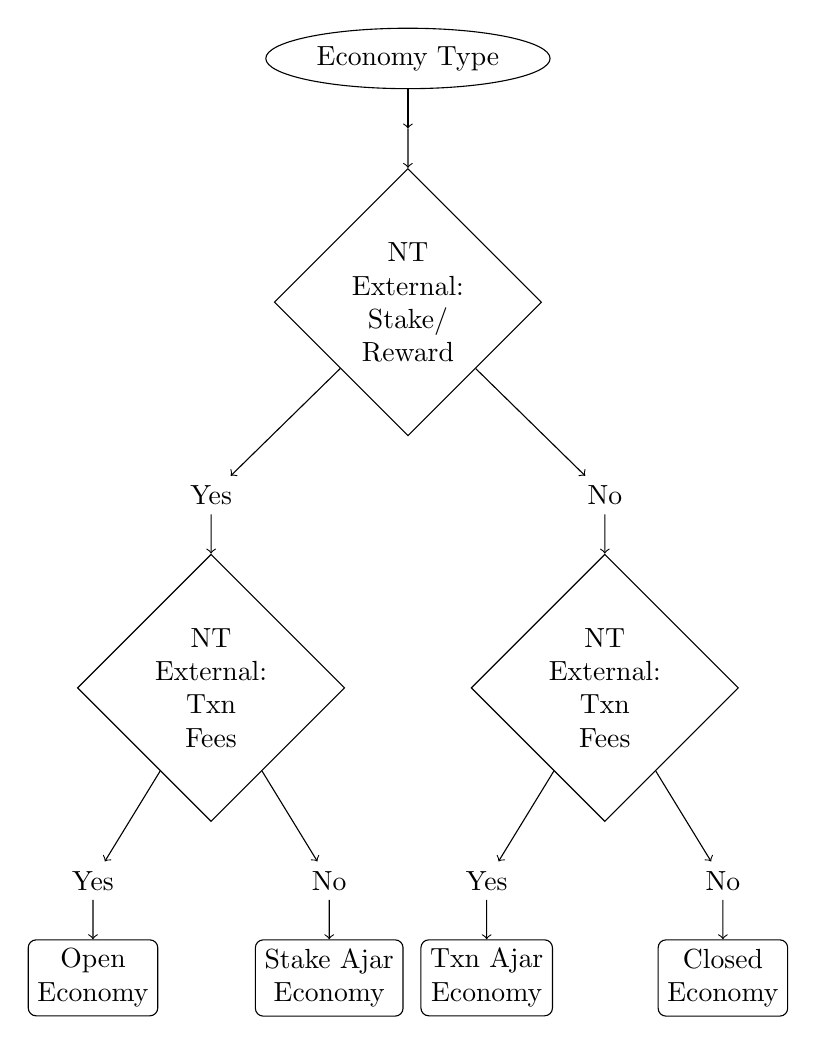
\begin{tikzpicture}[
    type/.style={ellipse, draw=black, rounded corners=1mm, fill=none,
        text centered, anchor=north, text=black},
    answer/.style={rectangle, draw=none, fill=none, text centered, anchor=north, text=black},
    question/.style={diamond, draw=black, fill=none, anchor=north, text=black},
    result/.style={rectangle, draw=black, rounded corners=1mm, fill=none,
        text centered, anchor=north, text=black},
    % fact/.style={rectangle, draw=none, rounded corners=1mm, fill=blue, drop shadow,
    %     text centered, anchor=north, text=white},
    % state/.style={diamond, draw=black, fill=none, anchor=north, text=black},
    % leaf/.style={circle, draw=none, fill=red, circular drop shadow,
    %     text centered, anchor=north, text=white},
    level distance=0.5cm, growth parent anchor=south
]
\node (Type00) [type] {Economy Type} [->]
    child{
        child{ [sibling distance=5cm]
            node (Q01) [question, align=center] {NT\\External:\\Stake/\\Reward}
            child{
                node (A02) [answer] {Yes}
                child{ [sibling distance=3cm]
                    node (Q02) [question, align=center] {NT\\External:\\Txn\\Fees}
                    child{
                        node (A03) [answer] {Yes}
                        child{
                            node (R03) [result, align=center] {Open\\Economy}
                        }
                    }
                    child{
                        node (A04) [answer] {No}
                        child{ [sibling distance=1.2cm]
                            node (R04) [result, align=center] {Stake Ajar\\Economy}
                        }
                    }
                }
            }
            child{ 
                node (A10) [answer] {No}
                child{ [sibling distance=3cm]
                    node (Q10) [question, align=center] {NT\\External:\\Txn\\Fees}
                    child{
                        node (A11) [answer] {Yes}
                        child{ 
                            node (R11) [result, align=center] {Txn Ajar\\Economy}
                        }
                    }
                    child{ 
                        node (A12) [answer] {No}
                        child{ 
                            node (R12) [result, align=center] {Closed\\Economy}
                        }
                    }
                }
            }
        }
    }   
;
        
\end{tikzpicture}
\caption{Token-Economy Economy Types} \label{fig:teet}
\end{figure}


\subsection{Model Type}
Reduced-form models establish relationships between endogenous variables based on observable variables. For example, an endogenous variable might be user adoption, proxied by observed daily active accounts. Structural models, on the other hand, originate from theories and provide a deeper understanding of behavioral patterns, which may involve unobservable parameters. The selection of an approach is frequently influenced by data availability and considerations related to estimation and calibration. In the absence of data, simulations are often employed as an alternative method.

\begin{figure}[H]
\small
\centering
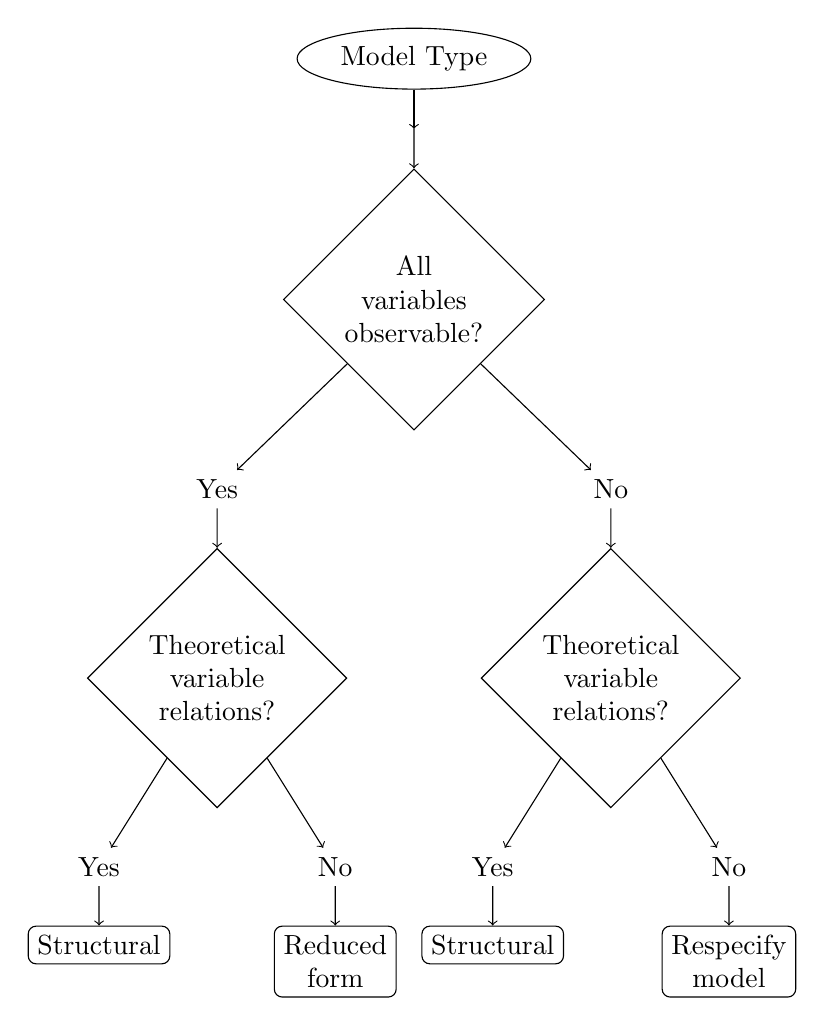
\begin{tikzpicture}[
    type/.style={ellipse, draw=black, rounded corners=1mm, fill=none,
        text centered, anchor=north, text=black},
    answer/.style={rectangle, draw=none, fill=none, text centered, anchor=north, text=black},
    question/.style={diamond, draw=black, fill=none, anchor=north, text=black},
    result/.style={rectangle, draw=black, rounded corners=1mm, fill=none,
        text centered, anchor=north, text=black},
    % fact/.style={rectangle, draw=none, rounded corners=1mm, fill=blue, drop shadow,
    %     text centered, anchor=north, text=white},
    % state/.style={diamond, draw=black, fill=none, anchor=north, text=black},
    % leaf/.style={circle, draw=none, fill=red, circular drop shadow,
    %     text centered, anchor=north, text=white},
    level distance=0.5cm, growth parent anchor=south
]
\node (Type00) [type] {Model Type} [->]
    child{
        child{ [sibling distance=5cm]
            node (Q01) [question, align=center] {All\\variables\\observable?}
            child{
                node (A02) [answer] {Yes}
                child{ [sibling distance=3cm]
                    node (Q02) [question, align=center] {Theoretical\\variable\\relations?}
                    child{
                        node (A03) [answer] {Yes}
                        child{
                            node (R03) [result, align=center] {Structural}
                        }
                    }
                    child{
                        node (A04) [answer] {No}
                        child{ [sibling distance=1.2cm]
                            node (R04) [result, align=center] {Reduced\\form}
                        }
                    }
                }
            }
            child{ 
                node (A10) [answer] {No}
                child{ [sibling distance=3cm]
                    node (Q10) [question, align=center] {Theoretical\\variable\\relations?}
                    child{
                        node (A11) [answer] {Yes}
                        child{ 
                            node (R11) [result, align=center] {Structural}
                        }
                    }
                    child{ 
                        node (A12) [answer] {No}
                        child{ 
                            node (R12) [result, align=center] {Respecify\\model}
                        }
                    }
                }
            }
        }
    }   
;
        
\end{tikzpicture}
\caption{Token-Economy Model Types} \label{fig:temt}
\end{figure}

\subsection{Equilibrium Type}
General equilibrium theory aims to provide an explanation of the behavior of supply, demand, and prices in an entire economy comprising multiple interacting markets. Its objective is to demonstrate that the interaction between demand and supply leads to an overall state of general equilibrium. This contrasts the theory of partial equilibrium, which focuses on analyzing a specific part of the economy while assuming other factors remain constant.

In a general equilibrium model, the overall equilibrium quantities and prices are determined endogenously for the entire economy. This involves considering initial endowments and modeling agent behavior, with the objective of describing changes in prices and quantities that result in a "Pareto Optimal" outcome. On the other hand, a partial equilibrium model focuses on analyzing a specific part of the economy while assuming other parts to be constant or even absent. In such cases, either the price or quantity process is typically specified, and the other variable is derived from it, which necessitates a reduced-form model. It is worth noting that a partial equilibrium approach can sometimes lead to outcomes where no trade occurs. When possible, it can be beneficial to calculate an equivalent structural equilibrium that supports a reduced-form partial equilibrium specification, and vice versa. 

\begin{figure}[H]
\small
\centering
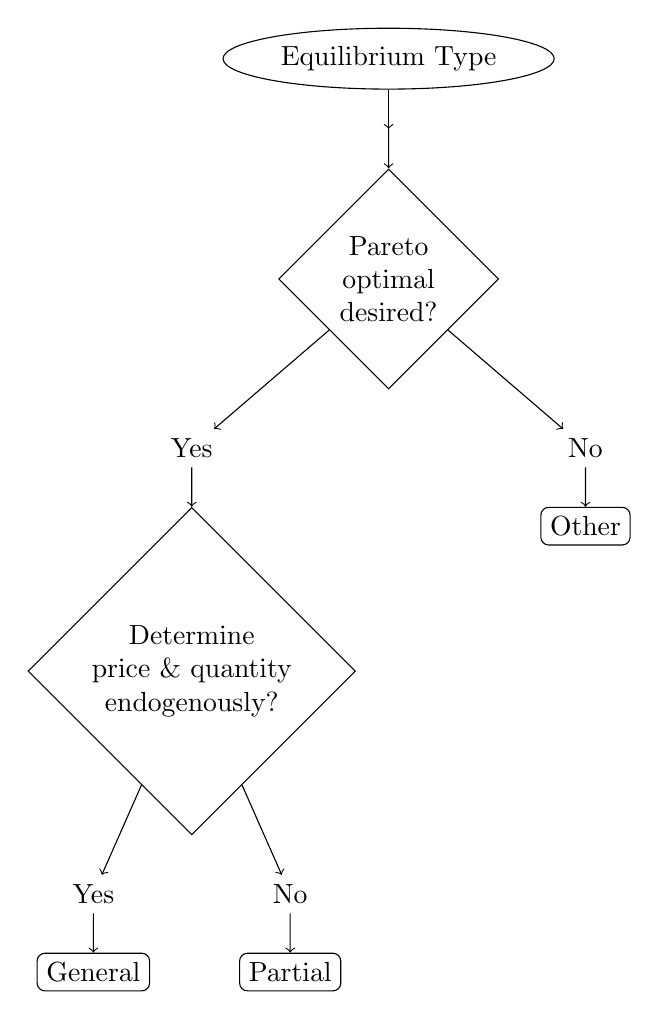
\begin{tikzpicture}[
    type/.style={ellipse, draw=black, rounded corners=1mm, fill=none,
        text centered, anchor=north, text=black},
    answer/.style={rectangle, draw=none, fill=none, text centered, anchor=north, text=black},
    question/.style={diamond, draw=black, fill=none, anchor=north, text=black},
    result/.style={rectangle, draw=black, rounded corners=1mm, fill=none,
        text centered, anchor=north, text=black},
    % fact/.style={rectangle, draw=none, rounded corners=1mm, fill=blue, drop shadow,
    %     text centered, anchor=north, text=white},
    % state/.style={diamond, draw=black, fill=none, anchor=north, text=black},
    % leaf/.style={circle, draw=none, fill=red, circular drop shadow,
    %     text centered, anchor=north, text=white},
    level distance=0.5cm, growth parent anchor=south
]
\node (Type00) [type] {Equilibrium Type} [->]
    child{
        child{ [sibling distance=5cm]
            node (Q01) [question, align=center] {Pareto\\optimal\\desired?}
            child{
                node (A02) [answer] {Yes}
                child{ [sibling distance=2.5cm]
                    node (Q02) [question, align=center] {Determine\\price \& quantity\\endogenously?}
                    child{
                        node (A03) [answer] {Yes}
                        child{
                            node (R03) [result, align=center] {General}
                        }
                    }
                    child{
                        node (A04) [answer] {No}
                        child{ [sibling distance=1.2cm]
                            node (R04) [result, align=center] {Partial}
                        }
                    }
                }
            }
            child{ 
                node (A10) [answer] {No}
                child{ [sibling distance=1.2cm]
                            node (R04) [result, align=center] {Other}
                }
            }
        }
    }   
;
\end{tikzpicture}
\caption{Token-Economy Equilibrium Types} \label{fig:teeqt}
\end{figure}


\subsection{Sector Type}
Multisector models are used to explore the allocation of resources across different activities, e.g. validator staking vs non-validator bonding. Commonly studied are consumption vs investment, public vs private, and real vs financial sectors. It is becoming more common to model more than two sectors, the number and character of each sector are either self-evident or too unique to be summarized in a decision tree.

\subsection{Production Type}
A production function is a specification of how the quantity of output behaves as a function of the inputs used in production.  In both general and partial equilibrium settings, it is used to connect different parts of an economy, for example, the Production-CAPM\autocite{cochrane91}.  Only two production functions are considered here: The Cobb-Douglas (C-D) and the Constant Elasticity of Substitution\footnote{Leontief, linear and Cobb–Douglas functions are special cases of the CES production function.} (CES).  The elasticity of substitution (ES) is a measure of how easy it is to shift between factor inputs - the percentage change in the ratio of the two inputs relative to the percentage change in their prices.

\begin{figure}[H]
\small
\centering
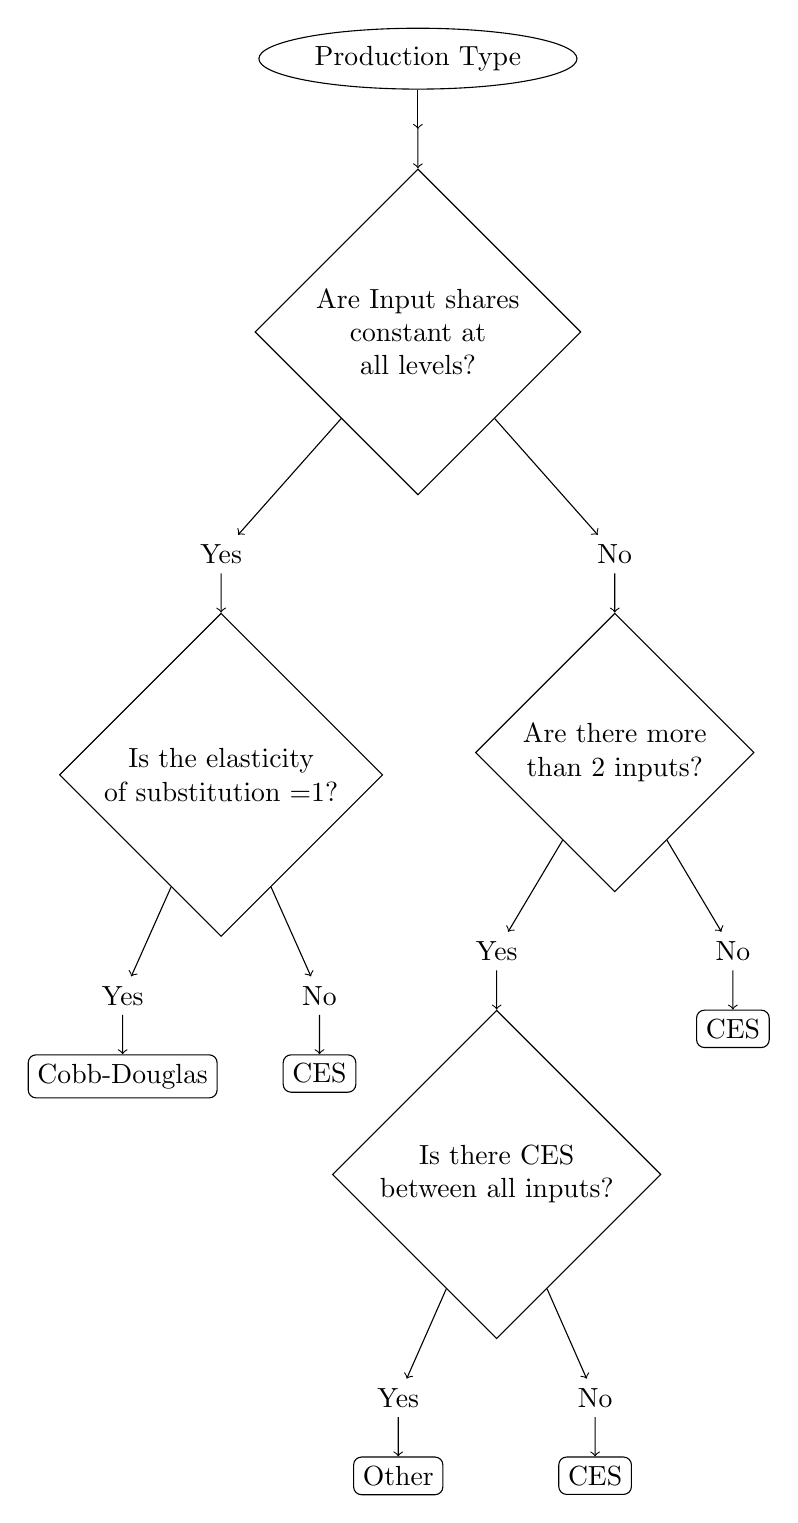
\begin{tikzpicture}[
    type/.style={ellipse, draw=black, rounded corners=1mm, fill=none,
        text centered, anchor=north, text=black},
    answer/.style={rectangle, draw=none, fill=none, text centered, anchor=north, text=black},
    question/.style={diamond, draw=black, fill=none, anchor=north, text=black},
    result/.style={rectangle, draw=black, rounded corners=1mm, fill=none,
        text centered, anchor=north, text=black},
    % fact/.style={rectangle, draw=none, rounded corners=1mm, fill=blue, drop shadow,
    %     text centered, anchor=north, text=white},
    % state/.style={diamond, draw=black, fill=none, anchor=north, text=black},
    % leaf/.style={circle, draw=none, fill=red, circular drop shadow,
    %     text centered, anchor=north, text=white},
    level distance=0.5cm, growth parent anchor=south
]
\node (Type00) [type] {Production Type} [->]
    child{
        child{ [sibling distance=5cm]
            node (Q01) [question, align=center] {Are Input shares\\constant at\\all levels?}
            child{
                node (A02) [answer] {Yes}
                child{ [sibling distance=2.5cm]
                    node (Q02) [question, align=center] {Is the elasticity\\of substitution =1?}
                    child{
                        node (A03) [answer] {Yes}
                        child{
                            node (R03) [result, align=center] {Cobb-Douglas}
                        }
                    }
                    child{
                        node (A04) [answer] {No}
                        child{ [sibling distance=1.2cm]
                            node (R04) [result, align=center] {CES}
                        }
                    }
                }
            }
            child{ 
                node (A11) [answer] {No}
                child{ [sibling distance=3cm]
                    node (Q10) [question, align=center] {Are there more\\than 2 inputs?}
                    child{
                        node (A02) [answer] {Yes}
                        child{ [sibling distance=2.5cm]
                            node (Q02) [question, align=center] {Is there CES\\between all inputs?}
                            child{
                                node (A03) [answer] {Yes}
                                child{
                                    node (R03) [result, align=center] {Other}
                                }
                            }
                            child{
                                node (A04) [answer] {No}
                                child{ [sibling distance=1.2cm]
                                    node (R04) [result, align=center] {CES}
                                }
                            }
                        }
                    }
                    child{ 
                        node (A12) [answer] {No}
                        child{ 
                            node (R12) [result, align=center] {CES}
                        }
                    }
                }
            }
        }
    }   
;
        
\end{tikzpicture}
\caption{Token-Economy Production Types} \label{fig:tept}
\end{figure}

\subsection{Monetary Type}
Monetary Policy is one of the most fraught topics in macroeconomics. There is no consensus on an unconditionally optimal policy. An important choice will be between adopting non-neutral or neutral monetary policies. While there is no consensus on the optimal choice, there is extensive literature on both. The monetary policy-related lectures for The Sveriges Riksbank Prize in Economic Sciences in Memory of Alfred Nobel\autocite{nobel}, provide a useful review of the background, progress, and controversies. Generally, the designer of a token economy will be left to choose from among the alternatives shown in Table~\ref{tbl:mpt}.

\begin{table}[H]
\caption{Monetary Policy Types} % title name of the table
\small
\centering % centering table
\begin{tabular}{l l l} % creating 3 columns
\hline\hline % inserting double-line
Monetary Target & Target Variable & Objective \\ [0.5ex]
\\ [0.5ex]
\hline % inserts single-line
Inflation & Interest rate & A given rate of change in an index \\
Price Level & Interest rate & A specific index number \\
Monetary Aggregate & Growth in money supply & A given rate of change in an index \\ 
Exchange Rate & The spot price of the currency & The spot price of the currency \\ 
Collateral peg & Collateral spot price & Low inflation as measured by the collateral price \\ 
\hline % inserts single-line

\end{tabular}
\label{tbl:mpt}
\end{table}

\subsection{Native Token Functions}

This analysis is limited to publicly available network whitepapers or token-economy/tokenomics documentation. None of the reviewed Polkadot parachain tokens were designed using a rational expectations framework (with the possible exception of the Equilibrium parachain), and none derive an expression for their token price dynamics. Consequently, the range of functionality for which tokens can be used has been summarized using the classification scheme by Burnie, Burnie, and Henderson(2018)\autocite{burnie18}.  In their scheme, differentiating tokens based on functional attributes, tokens are categorized into crypto-transaction tokens (cash substitutes); crypto-fuel tokens (generic blockchain applications); and crypto-voucher tokens (exchangeable for consumption goods). This classification helps identify issues to consider when participating in a cryptocurrency system.  For crypto-transaction and crypto-fuel tokens is the token a better form of money? For crypto-fuel tokens, the application user base and the utility of the token system are more important. For crypto-voucher tokens, the value of the numeraire good and the token’s exchangeability are important considerations.  The results are summarized in Table~\ref{tbl:ntf}.

\begin{table}[H]
\caption{Native Token Functions: Polkadot Ecosystem} % title name of the table
\small
\centering % centering table
\begin{tabular}{l l c c c} % creating 5 columns
\hline\hline % inserting double-line
Chain & Token & Fuel & Transaction & Voucher \\ [0.5ex]
\\ [0.5ex]
\hline % inserts single-line

% Entering 1st row
\rule{0pt}{1.5\normalbaselineskip}\href{\doturl}{Polkadot}     & DOT Y & Y & N & N \\
\href{\acaurl}{Acala}           & ACA       & Y & N & N \\
\href{\astrurl}{Astar}          & ASTR      & Y & N & N \\
\href{\bfcurl}{Bifrost}         & BFC       & Y & Y & N \\
\href{\cfgurl}{Centrifuge}      & CFG       & Y & N & N \\
\href{\clvurl}{Clover}          & CLV       & Y & Y & N \\
\href{\layrurl}{Composable}     & LAYR      & Y & N & N \\
\href{\cruurl}{Crust}           & CRU       & Y & Y & Y \\ 
\href{\ringurl}{Darwinia}       & RING      & Y & N & N \\ 
\href{\efiurl}{Efinity}         & EFI       & Y & N & N \\
\href{\equrl}{Equilibrium}      & EQ        & Y & Y & N \\
\href{\hdxurl}{HydraDX}         & HDX       & Y & N & N \\
\href{\intrurl}{Interlay}       & INTR      & Y & N & N \\
\href{\kilturl}{KILT}           & KILT      & Y & N & N \\
\href{\glmrurl}{Moonbeam}       & GLMR      & Y & N & N \\
\href{\nodlurl}{Nodle}          & NODL      & Y & N & N \\
\href{\tracotpurl}{OriginTrail} & TRAC/OTP  & Y & Y & N \\
\href{\paraurl}{Parallel}       & PARA      & Y & N & N \\
\href{\phaurl}{Phala}           & PHA       & Y & N & Y \\
\href{\dotsurl}{Statemint}      & DOT       & Y & N & N \\
\href{\unqurl}{Unique}          & UNQ       & Y & N & N \\[1.5ex]
% [1ex] adds vertical space
\hline % inserts single-line

\end{tabular}
\label{tbl:ntf}
\end{table}

\section{Token Price Models}

While the articles included here may be the first generation of Token pricing models, they nontheless encompass a reasonably broad range of Token characteristics and price dynamics. These are categorized as:

\begin{enumerate}
    \item \textbf{Effervescent-tokens:} \fullcite{cong21}
    \item \textbf{Dampened-tokens:} \fullcite{cong22}
    \item \textbf{Breakable-tokens:} \fullcite{sockin23a} and \fullcite{sockin23b}
    \item \textbf{Redeemable-tokens:} \fullcite{rogoff22}
\end{enumerate}

\section{Summary}

The annotated articles can be viewed in two ways. The first is a description of what platforms do. The second is a description of how platforms should be designed. Taking the first view, the results can help set expectations about platform functionality, strengths, and weaknesses. Taking the second view, the results can suggest how to configure a blockchain, point to possible users, and the functionality they may desire. As well as set expectations about the platform. Both views require mapping real-world properties and behaviors to abstract descriptions. And this requires an abundance of pragmatism and the willingness to live with approximations.

It is true that neither Polkadot nor the parachains currently on Polkadot have been designed nor conceived, using a rational expectations hypothesis.  That does not mean it is not possible to do so.  However, it is important to bear in mind that the models surveyed here are first-generation models. Consequently, it is very likely a blockchain that strives to implement one of the models described here will require substantial revisions as well as fine-tuning.

% Annotated Bibliography
\clearpage
\begin{refsection}[annotated_bibliography]
\nocite{long20,cong21,cong22,sockin23a,sockin23b,rogoff22}
\printbibliography[heading=bibnumbered]
\end{refsection}

\appendix
% \chapter*{Appendices}% If \appendix doesn't insert a \chapter
% \addcontentsline{toc}{chapter}{Appendices}% Print Appendix in ToC
% \setcounter{section}{0}% Reset numbering for sections
% \renewcommand{\thesection}{\Alph{section}}% Adjust section printing (from here onward)

\section{Methodology}
The published research annotated is six articles selected from the commercial research databases available from the State Library of New South Wales, Australia. The workflow and article counts are shown in Figure~\ref{fig:flowchart}.  This selection was arrived at in the following stages:
\begin{enumerate}
    \item Preparation:
    by operationalizing the inquiry \textit{"Refereed articles on block-chain token-economics using rational expectations equilibrium (a.k.a. no-arbitrage) arguments/analysis, ranked by journal impact factors"};
    \item Retrieval:
    eliminating duplicates;
    \item Screening:
    removing false positives;
    ranking by journal impact factor;
    \item Selection:
    selecting the top-6; and
    \item Write-up:
    reviewing remaining article abstracts and substituting where judged appropriate.
\end{enumerate}

\begin{figure}[!ht]
   \centering
   \begin{tabular}{c}
       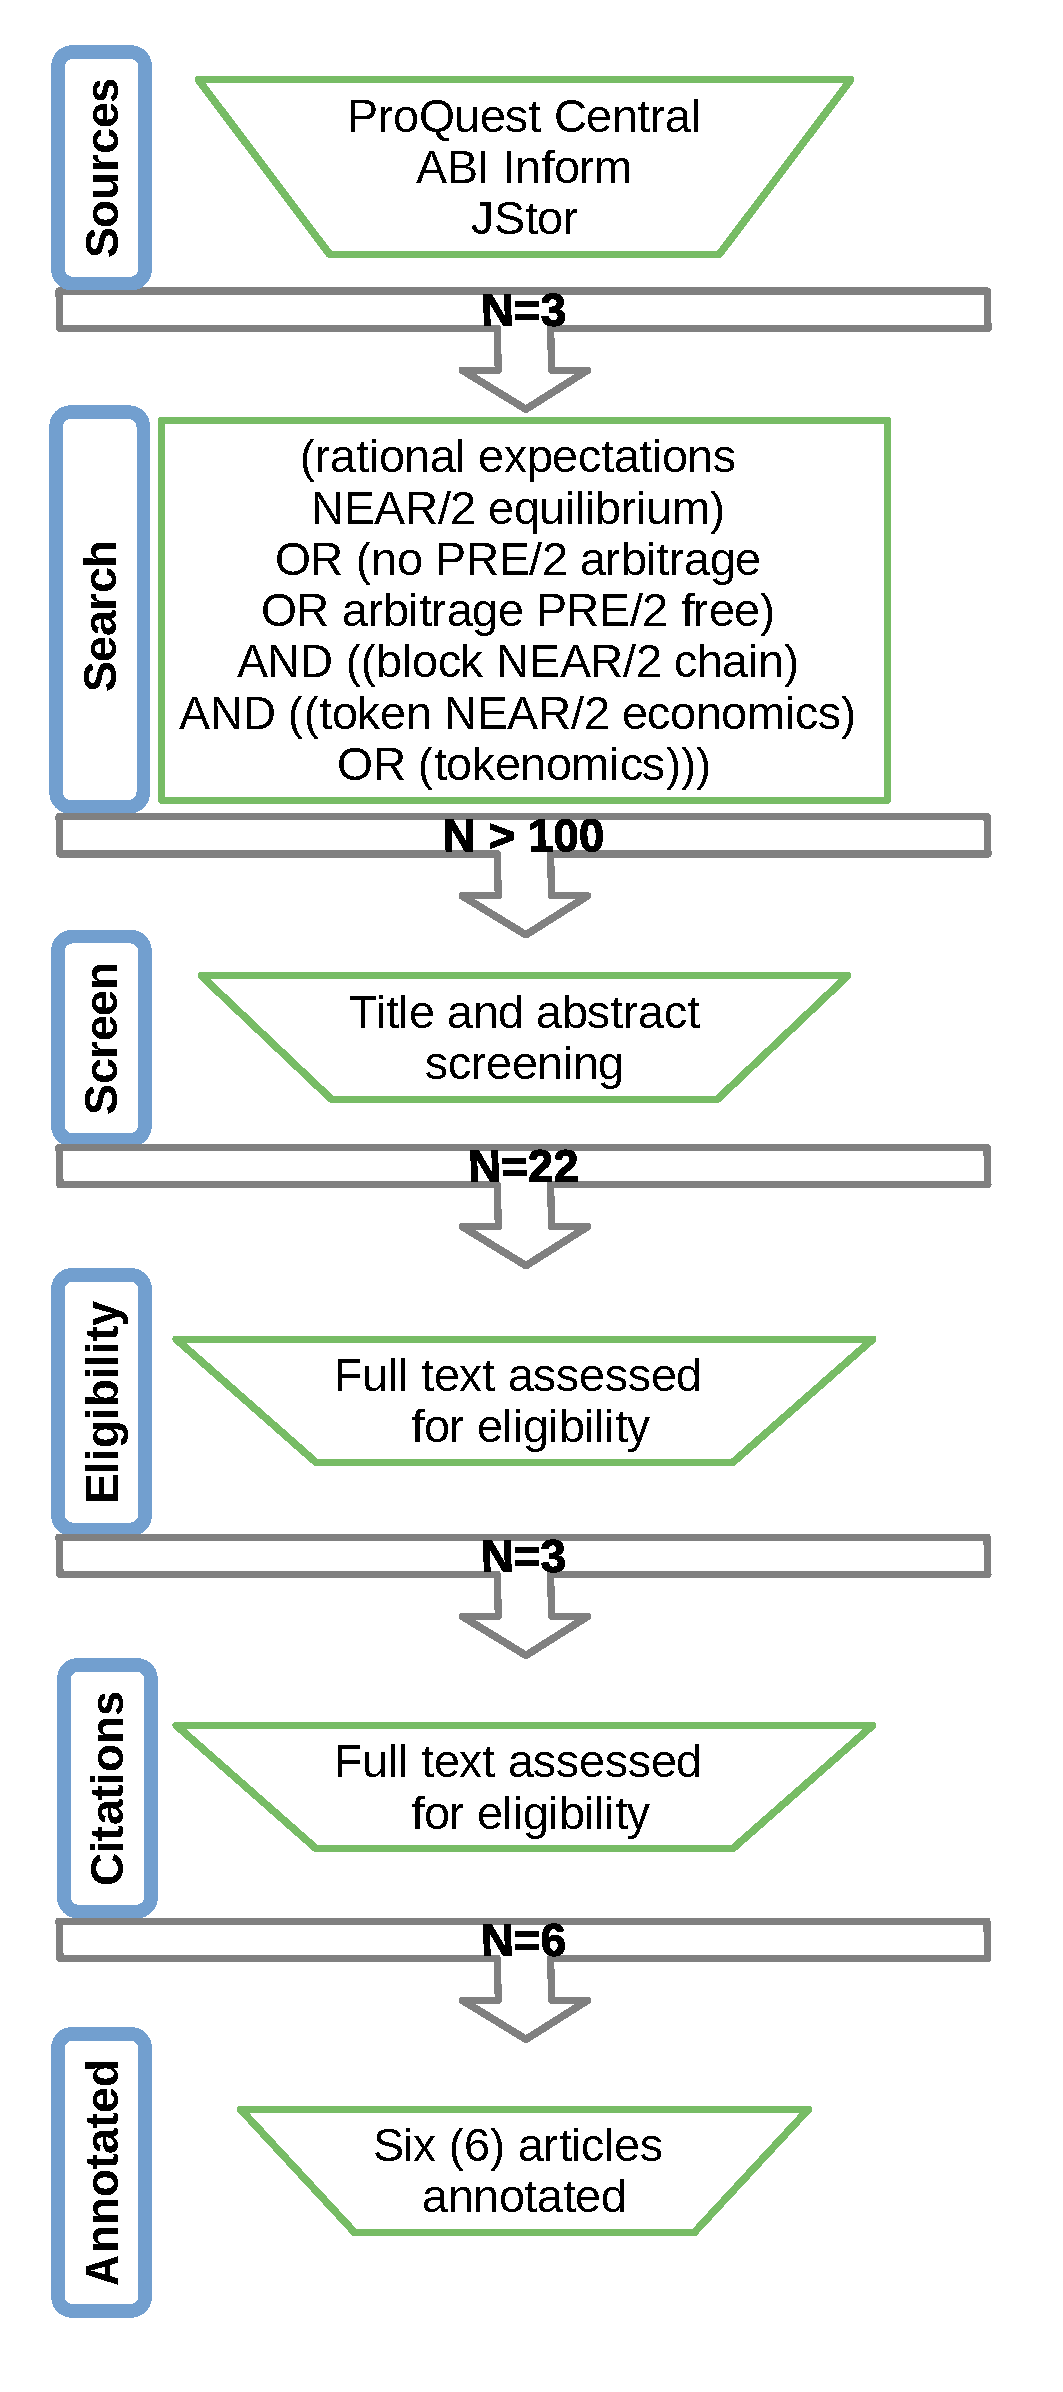
\includegraphics[page=1,width=.5\textwidth]{flowchart} 
   \end{tabular}
 \caption{Flowchart of the selection process.}
 \label{fig:flowchart}
\end{figure}

The annotated bibliography component of this project is closest to a "Scoping Review"\autocite{grant09}, and Table~\ref{tbl:sr}.

Each section of the report/working paper was developed using some subset of the following iterative process\autocite{tsafnat14}:
\begin{enumerate}
    \item Review reporting guidelines, best practice handbooks, and training modules [preparation stage]
    \item Formulate question and decide on review type [preparation stage]
    \item Search for previously published literature [preparation stage]
    \item Develop and test search strategies [preparation stage]
    \item Review search strategies [preparation stage]
    \item Execute search [retrieval stage]
    \item De-duplicate data/information [retrieval stage]
    \item Screen title and abstracts [screening stage]
    \item Retrieve full-text articles [retrieval stage]
    \item Screen articles in full-text [screening stage]
    \item Search for grey literature (preprints, working papers) [retrieval stage]
    \item Quality assessment and data/information extraction [synthesis stage]
    \item Citation chasing [retrieval stage]
    \item Update database searches [retrieval stage]
    \item Synthesize data/information [synthesis stage]
    \item Manuscript development [write-up stage]
\end{enumerate}

\end{document}

